\documentclass[12pt]{article}

\usepackage[top = 1in, bottom = 1in, left = 0.75in, right = 0.75in]{geometry}
\usepackage{amsmath, amssymb, amsthm}
\usepackage{graphicx}
\usepackage{float}

\theoremstyle{definition}
\newtheorem{question}{Question}
\newenvironment{answer}{
    \textbf{\textit{Answer:}} \qquad
}{\hfill $\blacksquare$ \\ \begin{center}
    \rule{0.6\linewidth}{0.5px}    
\end{center}
}


% CUSTOM DEFINITIONS
\newcommand{\R}{\mathbb{R}}
\newcommand{\Z}{\mathbb{Z}}
\newcommand{\C}{\mathbb{C}}


\title{Solution to Signal Processing Assignments I}
\author{Subhrajyoty Roy (MB1911)}
\date{\today}

\begin{document}
\maketitle

\begin{center}
    \rule{0.8\textwidth}{1px} 
\end{center}
\vspace*{2em}

% DONE
\begin{question}
    Determine if the following signals are energy signal or power signal or neither.
    \begin{enumerate}
        \item[(a)] $x(n) = 2\left(\dfrac{1}{3}\right)^n, \quad n > 0$.
        \item[(b)] $x(n) = u(n)$. 
    \end{enumerate}
\end{question}

\begin{answer}
    \begin{enumerate}
        \item[(a)]  Note that, the energy of the signal $x(n)$ is;
        \begin{align*}
            E_x & = \sum_{n = -\infty}^{\infty} (x(n))^2\\
            & = \sum_{n = 1}^{\infty} 4 \left(\dfrac{1}{3} \right)^{2n} \qquad \text{since, } x(n) = 0 \text{ if } n \leq 0\\
            & = 4\sum_{n = 1}^{\infty} (1/9)^n\\
            & = \dfrac{4}{9} \times \sum_{n = 0}^{\infty} (1/9)^n = \dfrac{4}{9} \times \dfrac{1}{(1 - (1/9))} = \dfrac{1}{2}
        \end{align*} 

        Thus the total energy of the given signal is finite, hence the given discrete time signal is an energy signal.

        \item[(b)] Since, $x(n) = u(n)$, which takes value $1$ if $n \geq 0$, otherwise take the value $0$, it is clear that, $(x(n))^2 = (u(n))^2 = u(n)$. Hence,
        
        $$
        E_x = \sum_{n = -\infty}^{\infty} (x(n))^2 = \sum_{n = -\infty}^{\infty} u(n) = \sum_{n = 0}^{\infty} 1 = \infty
        $$

        Clearly, the energy of the signal is not finite, hence the signal is not an energy signal. 

        To see whether this is a power signal, we consider;

        \begin{align*}
            P_x & = \lim_{N \rightarrow \infty} \dfrac{1}{(2N+1)} \sum_{n = -N}^N (x(n))^2\\
            & = \lim_{N \rightarrow \infty} \dfrac{1}{(2N+1)} \sum_{n = 0}^N u(n)\\
            & = \lim_{N \rightarrow \infty} \dfrac{(N+1)}{(2N + 1)} = \dfrac{1}{2}
        \end{align*}

        Hence, the power of the given signal $u(n)$ is finite, thus it is a power signal, but not an energy signal.
    \end{enumerate}
\end{answer}


% DONE
\begin{question}
    A discrete time system can be;
    \begin{enumerate}
        \item[(1)] Static or Dynamic
        \item[(2)] Linear or nonlinear
        \item[(3)] Time invariant or time varying
        \item[(4)] Causal or noncausal
        \item[(5)] Stable or unstable.   
    \end{enumerate}

    Examine the following systems with respect to the properties above.
\end{question}

\begin{answer}
    Let us denote any discrete time system by a generic symbol $\tau$. 
    \begin{enumerate}
        \item[(a)] $y(n) = \cos(x(n))$.
        
        The given system depends only on the current input value, but not on the past or future input values. Thus, the system is \textbf{Static}.

        The system is \textbf{nonlinear}, since,
        $$
        \cos(x_1(n) + x_2(n)) = \cos(x_1(n))\cos(x_2(n)) - \sin(x_1(n)) \sin(x_2(n)) \neq \cos(x_1(n)) + \cos(x_2(n)) 
        $$

        The system is \textbf{time-invariant}. Since, for any integer $k$, if the input is shifted by $k$ timesteps, the output shifts by the same amount, $\tau(x(n-k)) = \cos(x(n-k)) = y(n-k)$.

        The system is \textbf{causal}, as it depends only on the past and present (specifically only on the current) input values.

        The system is \textbf{BIBO Stable}, as for any integer $n$, $\vert y(n)\vert = \vert \cos(x(n)) \vert \leq 1$, i.e. the output is always bounded.


        \item[(b)] $y(n) = \sum_{k = -\infty}^{(n+1)}x(k)$.
         
        The output of this system depends on past values, current value of the input signal as well as one future value, as $y(n)$ depends on $x(n+1)$. Thus the system is \textbf{dyanmic} and \textbf{noncausal}.

        For any $\alpha, \beta \in \R$,

        \begin{align*}
            \tau(\alpha x_1(n) + \beta x_2(n))
            & = \sum_{k = -\infty}^{(n+1)} \left[ \alpha x_1(k) + \beta x_2(k) \right]\\
            & = \alpha \sum_{k = -\infty}^{(n+1)} x_1(k) + \beta \sum_{k = -\infty}^{(n+1)} x_2(k)\\
            & = \alpha \tau(x_1(n)) + \beta \tau(x_2(n))
        \end{align*}

        Thus, the system is \textbf{linear}.

        The system is also \textbf{time invariant}, since for any integer $n_0$,

        $$
        \tau(x(n-n_0)) = \sum_{k = -\infty}^{(n + 1)} x(k-n_0) =\sum_{l = -\infty}^{(n - n_0 + 1)} x(l) = y(n-n_0) 
        $$

        The system is \textbf{BIBO unstable}, as with $x(n) = u(n)$, which is bounded input, the output becomes $y(n) = (n+1)$ which is an unbounded sequence.

        \item[(c)] $y(n) = x(n) \cos(\omega_0 n)$. Clearly, the current input only depends on the current input, hence the system is \textbf{static} and \textbf{causal}. 
        
        The given system is also \textbf{linear}, as for any $\alpha, \beta \in \R$,

        $$
        \tau(\alpha x_1(n) + \beta x_2(n)) = (\alpha x_1(n) + \beta x_2(n)) \cos(\omega_0 n) = \alpha x_1(n)\cos(\omega_0 n) + \beta x_2(n) \cos(\omega_0 n)
        $$

        The system is \textbf{time varying}, as for any arbitrary integer $n_0$;

        $$
        \tau(x(n - n_0)) = x(n - n_0)\cos(\omega_0 n) \neq x(n - n_0)\cos(\omega_0 (n - n_0)) = y(n-n_0)
        $$

        and finally, the system is \textbf{BIBO stable}. Since, for any bounded input sequence $x(n)$ bounded by $M$, the output sequence $y(n)$ is also bounded by $M$ as;

        $$
        \vert y(n) \vert = \vert x(n) \vert \vert \cos(\omega_0 n) \vert \leq \vert x(n) \vert < M
        $$

        \item[(d)] $y(n) = x(-n+2)$.
        
        Note that, for $n = 0$, we have $y(0) = x(2)$, thus the current value of the output sequence may require the future input value. Hence, the system is \textbf{dynamic} and \textbf{noncausal}. However, the system is clearly \textbf{linear}.

        The system is \textbf{time varying}, as $y(0) = x(2)$ but $y(-1) = x(3)$, i.e. if the input sequence is shifted in the forward direction by $n_0$ timesteps, the output sequence is shifted in the backward direction by the same number of timesteps. This makes the system time varying.

        Finally, if the input sequence $x(n)$ is bounded by $M$, then the output sequence $y(n)$ is also bounded by $M$, thus the system is \textbf{stable}.
         
        \item[(e)] $y(n) = \text{Trun}[x(n)]$, where $\text{Trun}[x(n)]$ denotes the integer part of $x(n)$, obtained by truncation.
        
        Since the current output depends only on the current input, it is \textbf{static} and \textbf{causal}. 
        
        Now, consider a sequence $x(n)$ such that $x(0) = 1.6$. Then, 

        $$
        \tau(2x(0)) = \text{Trun}[2x(0)] = \text{Trun}[3.2] = 3 \neq 2 = 2 \times \text{Trun}[1.6] = 2 \tau(x(0)) 
        $$

        Hence, the system is \textbf{nonlinear}. 

        The system is clearly \textbf{time invariant}, as for any integer $n_0$, $\tau(x(n-n_0)) = \text{Trun}[x(n-n_0)] = y(n-n_0)$. The system is also BIBO \textbf{stable}, as for the input sequence bounded by $M$, the output sequence must satisfy;

        $$
        \vert y(n) \vert = \vert \text{Trun}[x(n)] \vert \leq \vert x(n) \vert < M
        $$

        \item[(f)] $y(n) = \text{Round}[x(n)]$, where $\text{Round}[x(n)]$ denotes the integer part of $x(n)$, obtained by rounding.
        
        Again, as the current output of the system depends only on the current input, it is \textbf{static} and \textbf{causal}. To see that the system is \textbf{nonlinear}, consider the same sequence $x(n)$ with $x(0) = 1.6$, so that;

        $$
        \tau(2x(0)) = \text{Round}[2x(0)] = \text{Round}[3.2] = 3 \neq 4 = 2\times 2 = 2 \times \text{Round}[1.6] = 2 \tau(x(0))
        $$

        By similar arguments of the previous solution (Q1 part (e)), it follows that the system is \textbf{time invariant}. The system is also BIBO \textbf{stable}, as for the input sequence bounded by $M$, the output sequence must satisfy;

        $$
        \vert y(n) \vert = \vert \text{Round}[x(n)] \vert \leq (\vert x(n) \vert + 1) < (M+1)
        $$     
        
        \item[(g)] $y(n) = \vert x(n)\vert$.
        
        Since the current output of the system depends only on the current input, the system is \textbf{static} and \textbf{causal}. The system is also \textbf{time invariant}. To see \textbf{BIBO stability} of the system, note that, for any bounded input sequence $x(n)$ bounded by $M$, the output sequence $y(n)$ has; $\vert y(n) \vert = \vert \vert x(n) \vert \vert = \vert x(n) \vert < M$, i.e. the output sequence is also bounded.

        However, the system is \textbf{nonlinear}. To see this, consider two sequences $x_1(n)$ and $x_2(n)$ such that, $x_1(0) = 5$ and $x_2(0) = (-5)$. Then,

        $$
        \tau(x_1(0) + x_2(0)) = \vert 5 + (-5) \vert = 0 \neq 10 = \vert 5 \vert + \vert (-5) \vert = \tau(x_1(0)) + \tau(x_2(0))
        $$

        \item[(h)] $y(n) = x(n) u(n)$.
        
        The system is \textbf{static} and \textbf{causal}, since the current output only depends on the current input value. 

        The system is \textbf{linear}, since for any $\alpha, \beta \in \R$, we have;

        $$
        \tau(\alpha x_1(n) + \beta x_2(n)) = (\alpha x_1(n) + \beta x_2(n)) u(n) = \alpha x_1(n)u(n) + \beta x_2(n)u(n) = \alpha \tau(x_1(n)) + \beta \tau(x_2(n))
        $$

        The system is also \textbf{BIBO stable}, since for any bounded input sequence $x(n)$ bounded by $M$, the output sequence $y(n)$ satisfy; $\vert y(n) \vert = \vert x(n) u(n) \vert \leq \vert x(n) \vert < M$.

        Finally, the system is \textbf{time varying}. For instance, consider the input signal $x(n) = [1, 2, \underset{\uparrow}{3}, 4, 5]$. Then, the output signal $y(n) = [0, 0, \underset{\uparrow}{3}, 4, 5]$. Now, assume that the input signal is shifted so that we now feed the signal $x'(n) = [1, 2, 3, \underset{\uparrow}{4}, 5]$. Then, the output would come out to be $[0, 0, 0, \underset{\uparrow}{4}, 5]$, which is the a shifted version of $y(n)$ (as $y(0)$ was equal to $3$ beforehand).

        \item[(i)] $y(n) = x(n) + nx(n+1)$.
        
        The current output of the system depends on the current input $x(n)$ as well as it anticipates the next input $x(n+1)$, hence the system is \textbf{dynamic} and \textbf{noncausal}. 

        The system is \textbf{linear}, as for any $\alpha, \beta \in \R$, and for any input sequences $x_1(n)$ and $x_2(n)$, we have;

        \begin{align*}
            \tau(\alpha x_1(n) + \beta x_2(n)) 
            & = (\alpha x_1(n) + \beta x_2(n)) + n (\alpha x_1(n+1) + \beta x_2(n+1))\\
            & = \alpha (x_1(n) + n x_1(n+1)) + \beta (x_2(n) + n x_2(n+1))\\
            & = \tau(x_1(n)) + \tau(x_2(n))      
        \end{align*}

        The system is \textbf{time varying}. To see this, consider an input sequence $x(n) = [\underset{\uparrow}{1}, 2, 3]$. Then, the output sequence would be; $y(n) = [-1, \underset{\uparrow}{1}, 5, 3]$. Now consider shifting the input sequence by $1$ timeunits, so that we have $x'(n) = [1, \underset{\uparrow}{2}, 3]$ as the input. Then, the resulting output sequence becomes $y'(n) = [-2, -1, \underset{\uparrow}{2}, 3]$, which is not the shifted version of $y(n)$.

        The system is \textbf{BIBO unstable}. For example, consider the input sequence $x(n) = u(n)$ which is clearly a bounded sequence, but then for $n \geq 0$, $y(n) = u(n) + n u(n + 1) = (1 + n)$, which is an unbounded sequence.

        \item[(j)] $y(n) = x(2n)$.
        
        The system is \textbf{dynamic} and \textbf{noncausal}, as $y(1)$ depends on $x(2)$, the input of a future time point. However, the system is clearly \textbf{linear}. 
        
        The given system is \textbf{time varying}. For example, consider the input sequence $x(n) = [\underset{\uparrow}{1}, 2, 3, 4]$ whose output is $y(n) = [\underset{\uparrow}{1}, 3]$. Now with a shifted input $[1, \underset{\uparrow}{2}, 3, 4]$, the output becomes $[2, 4]$, which is not the shifted version of $y(n)$.

        However, the system remains \textbf{BIBO stable}, since if there exists $M$ such that $\vert x(n) \vert < M$ for any integer $n$, then clearly, $\vert y(n) \vert = \vert x(2n) \vert < M$, i.e. the output sequence is also bounded.

        \item[(k)] $y(n) = \begin{cases}
            x(n) & \text{ if } x(n) \geq 0\\
            0 & \text{ if } x(n) < 0
        \end{cases}$

        The current output of the system depends only on the current input, thus the system is \textbf{static} and \textbf{causal}. 

        The system is \textbf{nonlinear}. For example, if $x_1(n) = [\underset{\uparrow}{3}, 4, -1, -1]$ and $x_2(n) = [\underset{\uparrow}{-2}, -2, 4, 3]$, then, 

        $$
        \tau(x_1(n) + x_2(n)) = \tau([\underset{\uparrow}{1}, 2, 3, 2]) = [\underset{\uparrow}{1}, 2, 3, 2]
        $$

        while

        $$
        \tau(x_1(n)) + \tau(x_2(n)) = [\underset{\uparrow}{3}, 4, 0, 0] + [\underset{\uparrow}{0}, 0, 4, 3] = [\underset{\uparrow}{3}, 4, 4, 3]
        $$

        which are not equal to each other.

        The system is \textbf{time invariant}. For any integer $n_0$, if the input sequence is shifted by $n_0$ timesteps, then;

        $$
        \tau(x(n-n_0)) = \max\{ 0, x(n-n_0) \} = y(n-n_0)
        $$

        Finally, the system is also \textbf{BIBO stable}, since if the input sequence $x(n)$ is bounded by some number $M$ then, $\vert y(n) \vert \leq \vert x(n) \vert < M$, i.e. the output sequence is also bounded by the same number.

        \item[(l)] $y(n) = x(-n)$.
        
        Since $y(-1) = x(1)$, i.e. the current output anticipates the future input, the system is \textbf{dynamic} and \textbf{noncausal}.

        Clearly, the system is \textbf{linear}.

        To see that the system is \textbf{time varying}, consider the sequence $x(n) = [\underset{\uparrow}{1}, 2, 3]$, which outputs the sequence $y(n) = [3, 2, \underset{\uparrow}{1}]$. On the other hand, with a shifted input $[1, \underset{\uparrow}{2}, 3]$, the output becomes $[3, \underset{\uparrow}{2}, 1]$, where the shift appears in the reverse direction. To see this, note that for any integer $n_0$, $\tau(x(n-n_0)) = x(-(n-n_0)) = x(-n + n_0) = y(n + n_0)$.

        Finally, the system is obviously \textbf{BIBO stable}, since the number $M$ which bounds the input signal also serves as a bound to the output signal.

        \item[(m)] $y(n) = \text{sign}(x(n))$.
        
        The current output of the system depends only on the current input, hence the system is \textbf{static} and \textbf{causal}. Also, the system is \textbf{BIBO stable}, as for any bounded input sequence $x(n)$, $y(n)$ takes values in the set $\{ -1, 0, 1 \}$, which is bounded.

        The system is \textbf{nonlinear}, since we can consider two sequences $x_1(n)$ and $x_2(n)$ with $x_1(0) = 2$ and $x_2(0) = (-1)$ respectively. Then,

        $$
        \tau(x_1(0) + x_2(0)) = \text{sign}(2-1) = 1 \neq 0 = (+1 - 1) = \text{sign}(2) + \text{sign}(-1) = \tau(x_1(0)) + \tau(x_2(0))
        $$

        Finally, the system is obviously \textbf{time invariant}. Since, for any integer $n_0$, $\tau(x(n-n_0)) = \text{sign}(x(n-n_0)) = y(n-n_0)$.

        \item[(n)] The ideal sampling system with input $x_a(t)$ and output $x(n) = x_a(nT)$ for $-\infty < n < \infty$.  
        
        If the sampling period $T < 1$, then the current output depends only on the past input of the analogue signal, as $nT < n$. If the sampling period $T = 1$, then the current output is same as the current input of the analogue signal as $nT = n$. If $T > 1$, then the current output anticipates a future input of the analogue signal as $nT > n$.

        Thus,

        $$
        \text{The given system is } \begin{cases}
            \text{\textbf{causal} and \textbf{dynamic} if } T < 1\\
            \textbf{\textbf{causal} and \textbf{static} if } T = 1\\
            \textbf{\textbf{noncausal} and \textbf{dynamic} if } T > 1\\
        \end{cases}
        $$

        The system is clearly \textbf{linear}, as for any $\alpha, \beta \in \R$ and arbitrary analogue signals $x_{1a}(t)$ and $x_{2a}(t)$, we have for any integer $n$;

        $$
        \tau(\alpha x_{1a}(t) + \beta x_{2a}(t))(n) = \alpha x_{1a}(nT) + \beta x_{2a}(nT) = \alpha \tau(x_{1a}(t))(n) + \beta \tau(x_{2a}(t))(n)
        $$

        The system is \textbf{time invariant}. Consider the $t_0$ time delayed input signal $x'_a(t) = \cos(\omega(t - t_0))$ of the original signal $x_a(t) = \cos(\omega t)$. The output of the sampling system on the time delayed version would be $x'(n) = \cos(\omega(nT - t_0))$, which is the delayed version of the signal $\cos(\omega (nT))$, i.e. the output of the sampling system with input $x_a(t)$.

        Finally the system is clearly \textbf{BIBO stable}, since if the input analogue signal is bounded by some number $M$ then the same bound holds for the output digital signal as well.
    \end{enumerate}
\end{answer}


% DONE
\begin{question}
    Consider a signal $x(n) = [-3, 1, \underset{\uparrow}{2}, -2, 3, -1]$. Manually sketch the following signals:

    \begin{enumerate}
        \item[(a)] $x(n)$
        \item[(b)] $x(2-n)$
        \item[(c)] $x\left(\dfrac{2}{3}n + 1\right)$  
    \end{enumerate}
\end{question}

\begin{answer}
    \begin{enumerate}
        \item[(a)] The discrete time signal $x(n)$ looks as follows:
        \begin{figure}[H]
            \centering
            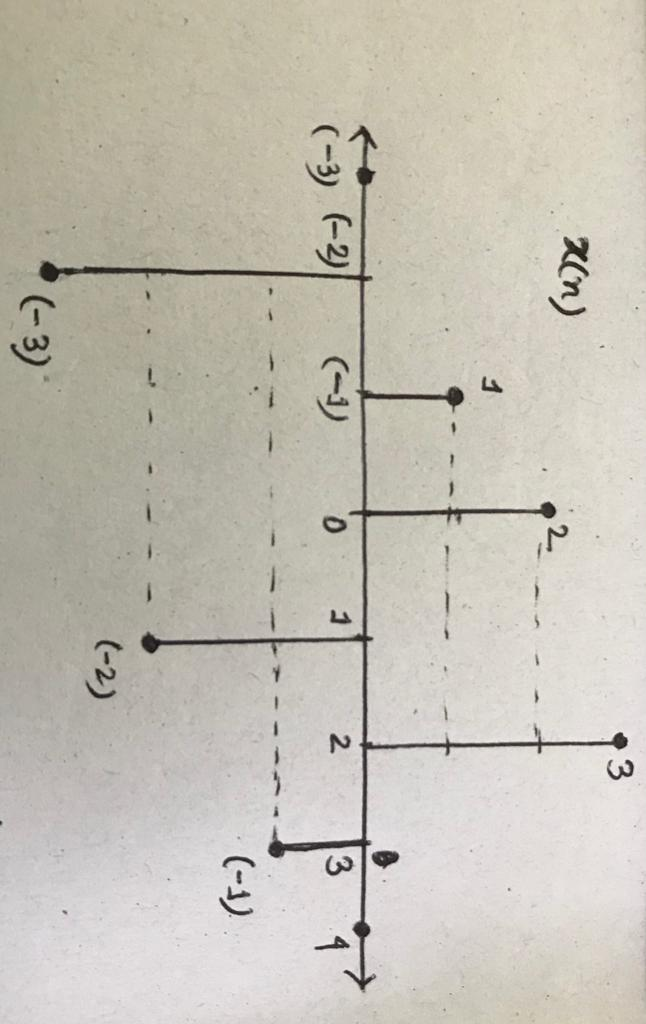
\includegraphics[height = 0.5\linewidth, angle = 90]{q3_a.jpeg}
        \end{figure} 
        \item[(b)] The discrete time signal $x(2-n)$ is simply a shifted version of the fold of $x(n)$. It is, $x(2-n) = [-1, \underset{\uparrow}{3}, -2, 2, 1, -3]$. The sketch is shown below.
        \begin{figure}[H]
            \centering
            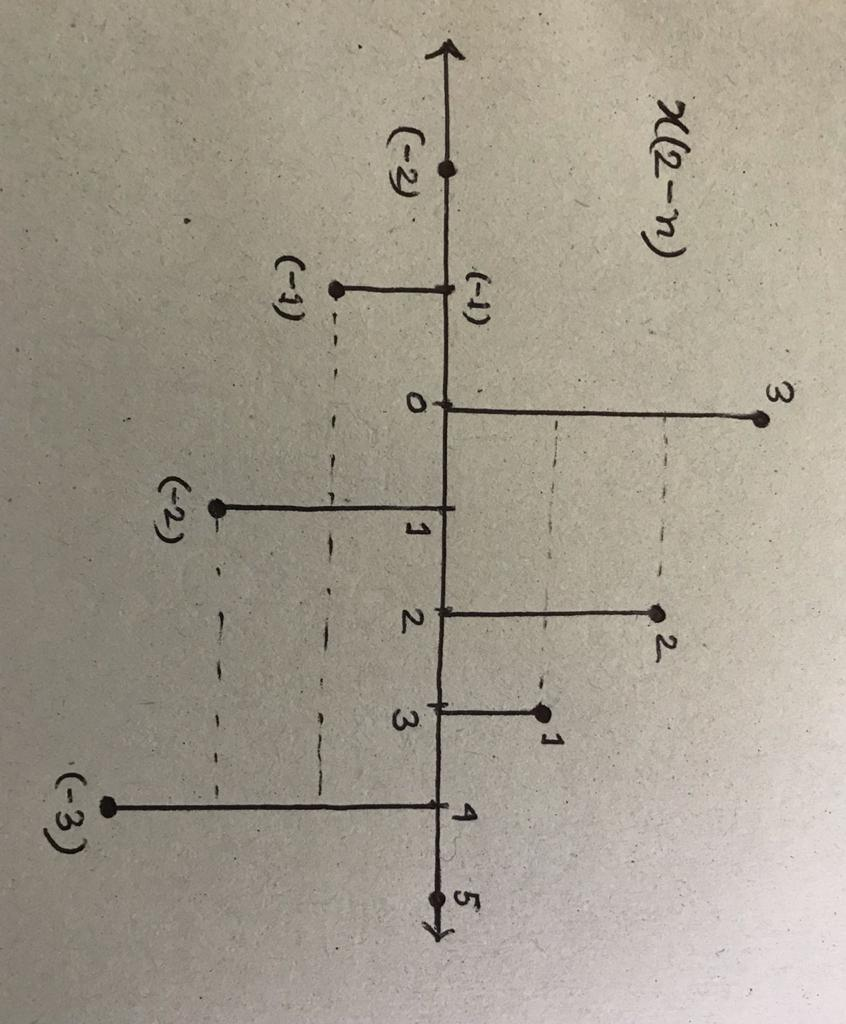
\includegraphics[height = 0.5\linewidth, angle = 90]{q3_b.jpeg}
        \end{figure}  
        \item[(c)] In this case assuming the sampling interval remaining same, only values where $\left( \dfrac{2}{3}n + 1\right)$ is an integer will be sampled. Thus, we must have, $\dfrac{2}{3}n$ as an integer (i.e. $n$ is a multiple of $3$) to possibly have any non-zero value for the signal. Note that, at $n = 0$, the value of the signal is $x(1)$, at $n = 3$, the value of the signal is $x(3)$ and at $n = (-3)$, the value of the signal is equal to $x(-1)$. 
        \begin{figure}[H]
            \centering
            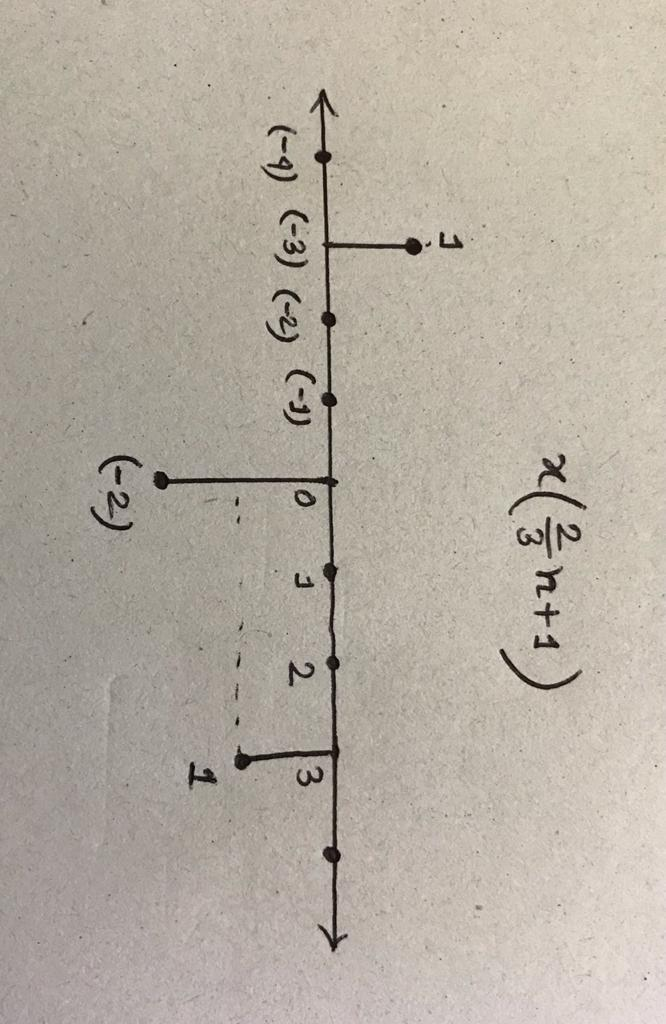
\includegraphics[height = 0.5\linewidth, angle = 90]{q3_c.jpeg}
        \end{figure}   
    \end{enumerate}
\end{answer}

% DONE
\begin{question}
    For the systems with input $x(n)$ and output $y(n)$, determine whether these are: (i) linear; (ii) time-invariant; (iii) causal.
    \begin{enumerate}
        \item[(a)] $y(n) = \log[x(n)]$.
        \item[(b)] $y(n) = x(n)x(n-2)$.
        \item[(c)] $y(n) = \sum_{k=0}^n x(k)$.
        \item[(d)] $y(n) = \sum_{k = -\infty}^n x(k)$.   
    \end{enumerate}
\end{question}

\begin{answer}
    Let $\tau$ be a generic symbol of any discrete time system.
    \begin{enumerate}
        \item[(a)] The given system is \textbf{nonlinear}. Too see this, let $x_1(n), x_2(n)$ be two discrete time signals;
        $$
        \tau(x_1(n) + x_2(n)) = \log[x_1(n) + x_2(n)] \neq \log[x_1(n)x_2(n)] = \log[x_1(n)] + \log[x_2(n)] = \tau(x_1(n)) + \tau(x_2(n))
        $$ 

        The system is clearly \textbf{time invariant}, as for any integer $n_0$, $\tau(x(n-n_0)) = \log[x(n-n_0)] = y(n-n_0)$. The system is also \textbf{causal}, as the current output depends only on the current and past inputs (specifically only the current inputs).

        \item[(b)] Note that, for some arbitrary discrete time signals $x_1(n)$ and $x_2(n)$;
        \begin{align*}
            \tau(x_1(n) + x_2(n))
            & = (x_1(n) + x_2(n))(x_1(n-2) + x_2(n-2))\\
            & \neq x_1(n)x_1(n-2) + x_2(n)x_2(n-2)\\
            & = \tau(x_1(n)) + \tau(x_2(n))
        \end{align*} 
        Hence, the given system is \textbf{nonlinear}.

        However, the system is \textbf{causal} and \textbf{time-invariant}. Clearly, the current output of the system only depends on the current input $x(n)$ and one past input $x(n-2)$. To see time-invariance property, note that for any integer $n_0$;
        $$
        \tau(x(n-n_0)) = x(n-n_0)x(n - n_0 - 2) = y(n-n_0)
        $$
        \item[(c)] The system is clearly \textbf{linear}. Since, for any $\alpha, \beta \in \R$;
        $$
        \tau(\alpha x_1(n) + \beta x_2(n)) = \sum_{k = 0}^{n} \left( \alpha x_1(k) + \beta x_2(k) \right) = \alpha \sum_{k = 0}^{n} x_1(k) + \beta \sum_{k = 0}^{n} x_2(k) = \alpha \tau(x_1(k)) + \beta \tau(x_2(k))
        $$ 

        Current output of the system depends only on the past inputs, thus the system is \textbf{causal}. However, the system is \textbf{time varying}. For example, consider the sequence $x(n) = [-1, \underset{\uparrow}{1}, 2, 3]$. Clearly, $y(n) = [\underset{\uparrow}{1}, 3, 6]$. Now note that, if we shift the input sequence by 1 unit of time we get $Sh_1(x(n)) = [-1, 1, \underset{\uparrow}{2}, 3]$. Hence, the system applied on this shifted sequence outputs $y'(n) = [\underset{\uparrow}{2}, 5]$, which is not equal to the 1 unit shifted version of $y(n)$.
        \item[(d)] Similar to part (c), it is easy to establish that the system is \textbf{linear} and \textbf{causal}. To see that the system is \textbf{time-invariant}, note that, for any integer $n_0$;
        $$
        \tau(x(n-n_0)) = \sum_{k = -\infty}^{(n)} x(k-n_0) =\sum_{l = -\infty}^{(n - n_0)} x(l) = y(n-n_0) 
        $$  
    \end{enumerate}
\end{answer}


% DONE
\begin{question}
    For LTI with the impulse reposnse function $h(n)$, find if the following systems are (i) causal, (ii) BIBO stable.
    \begin{enumerate}
        \item[(a)] $h(n) = \left(\dfrac{3}{4}\right)^n u(n-1)$.
        \item[(b)] $h(n) = 2^n u(-n + 1)$. 
    \end{enumerate}
\end{question}

\begin{answer}
    \begin{enumerate}
        \item[(a)] We know that an LTI system is causal if its unit impulse response sequence $h(n)$ satisfies that $h(n) = 0$ for any $n < 0$. Clearly, for the given system, $h(n) = 0$ for any $n < 1$, as then $(n-1) < 0$ and $u(n-1) = 0$. 
        
        For an LTI system to be BIBO stable, we require that its unit impulse reposnse sequence must be absolutely summable. In this case, since $u(n-1) > 0$ only if $n \geq 1$, we have;

        $$
        \sum_{n = -\infty}^{\infty} \vert h(n) \vert = \sum_{n = 1}^{\infty} \left(\dfrac{3}{4}\right)^n = \dfrac{3}{4} \sum_{n = 0}^{\infty} \left(\dfrac{3}{4}\right)^n = \dfrac{3}{4} \dfrac{1}{(1 - (3/4))} = 3
        $$

        Thus, the given LTI system is \textbf{causal} and \textbf{BIBO stable}.
        \item[(b)] Note that, 
        $$h(-1) = 2^{-1} u(-(-1) + 1) = \dfrac{1}{2} u(2) = \dfrac{1}{2} \neq 0$$   

        On the other hand, for the absolute summability;

        \begin{align*}
            \sum_{n = -\infty}^{\infty} \vert h(n) \vert 
            & = \sum_{n = -\infty}^{\infty} 2^n u(-n + 1)\\
            & = \sum_{m = -\infty}^{\infty} 2^{-m} u(m + 1)\\
            & = \sum_{m = -1}^{\infty} 2^{-m} \qquad \text{since, } u(m + 1) > 0 \text{ if and only if } m \geq (-1)\\
            & = 2 + \dfrac{1}{(1 - 1/2)} = 4 
        \end{align*}

        Thus the given LTI system is \textbf{noncausal} and \textbf{BIBO stable}.
    \end{enumerate}
\end{answer}


\begin{question}
    For each of the system below, determine whether the system is linear and/or shift-invariant.
    \begin{enumerate}
        \item[(a)] $y(n) = 2x(n) + 3$.
        \item[(b)] $y(n) = x(n) \sin\left( \dfrac{2\pi}{7}n + \dfrac{\pi}{6} \right)$.
        \item[(c)] $y(n) = (x[n])^2$
        \item[(d)] $y(n) = \sum_{m = -\infty}^n x(m)$   
    \end{enumerate}
\end{question}

\begin{answer}
    Let $\tau$ be a generic symbol for any discrete time system.
    \begin{enumerate}
        \item[(a)] The given system is \textbf{nonlinear} and \textbf{time invariant}.
        
        Note that, for any arbitrary $x_1(n)$ and $x_2(n)$, 

        $$
        \tau(x_1(n) + x_2(n)) = 2(x_1(n) + x_2(n)) + 3 \neq (2 x_1(n) + 3) + (2 x_2(n) + 3) = \tau(x_1(n)) + \tau(x_2(n))
        $$

        This shows that the system is nonlinear. To see time invariancy of the system, consider a delayed input to the system for any delay $n_0$.

        $$
        \tau(x(n - n_0)) = 2x(n - n_0) + 3 = y(n - n_0)
        $$

        \item[(b)] The given system is \textbf{linear}. Consider any arbitrary sequences $x_1(n), x_2(n)$ and any real numbers $\alpha, \beta \in \R$;
        
        \begin{align*}
            \tau(\alpha x_1(n) + \beta x_2(n)) 
            & = (\alpha x_1(n) + \beta x_2(n)) \sin\left( \dfrac{2\pi}{7}n + \dfrac{\pi}{6} \right)\\
            & = \alpha x_1(n) \sin\left( \dfrac{2\pi}{7}n + \dfrac{\pi}{6} \right) + \beta x_2(n) \sin\left( \dfrac{2\pi}{7}n + \dfrac{\pi}{6} \right)\\
            & = \tau(x_1(n)) + \tau(x_2(n))            
        \end{align*}

        However, the system is \textbf{time varying}. Since, the $n_0$-delayed output sequence is $y(n - n_0) = x(n-n_0) \sin\left( \dfrac{2\pi}{7}(n - n_0) + \dfrac{\pi}{6} \right)$, while the output of the delayed input $x(n - n_0)$ will be $x(n - n_0)\sin\left( \dfrac{2\pi}{7}n + \dfrac{\pi}{6} \right)$. Hence, as long as $\dfrac{2\pi}{7}n_0$ is not an integral multiple of $2\pi$, the above output sequences would not be same.

        \item[(c)] The system is \textbf{nonlinear}, as
        
        \begin{align*}
            \tau(x_1(n) + x_2(n)) & = (x_1(n) + x_2(n))^2\\
            & = x_1^2(n) + x_2^2(n) + 2x_1(n)x_2(n) \\
            & \neq x_1^2(n) + x_2^2(n) = \tau(x_1(n)) + \tau(x_2(n))            
        \end{align*}

        The system is \textbf{time invariant}. For any integer $n_0$;

        $$
        \tau(x(n - n_0)) = x^2(n - n_0) = y(n - n_0)
        $$

        \item[(d)] The given system is \textbf{linear} and \textbf{time invariant}. The reason is explained in detail in the solution of Question 4(d).



    \end{enumerate}
\end{answer}



% DONE
\begin{question}
    For each pair of input sequence $x(n)$ and unit impulse reposnse $h(n)$ of an LTI system, determine the output sequence $y(n)$. Sketch your results.
\end{question}

\begin{answer}
    We know that any LTI system's output is characterized by a discrete convolution of the input signal with the unit impulse reponse of the system. Thus, $y(n) = (h \ast x)(n)$, where $\ast$ denotes the discrete convolution operation.
    \begin{enumerate}
        \item[(a)] We are given;
        $$
        x(n) = [\underset{\uparrow}{1}, 2, 1] \qquad h(n) = u(n)
        $$ 
        So, we have;
        \begin{align*}
            y(n) 
            & = (h \ast x)(n) \\
            & = \sum_{k = -\infty}^{\infty} x(k)h(n-k)\\
            & = x(0)u(n) + x(1)u(n-1) + x(2)u(n-2)\\
            & = u(n) + 2u(n-1) + u(n-2)
        \end{align*} 

        In other words,
        $$
        y(n) = \begin{cases}
            0 & n < 0\\
            1 & n = 0\\
            3 & n = 1\\
            4 & n \geq 2\\
        \end{cases}
        $$

        The sketch of the output signal is as follows:

        \begin{figure}[H]
            \centering
            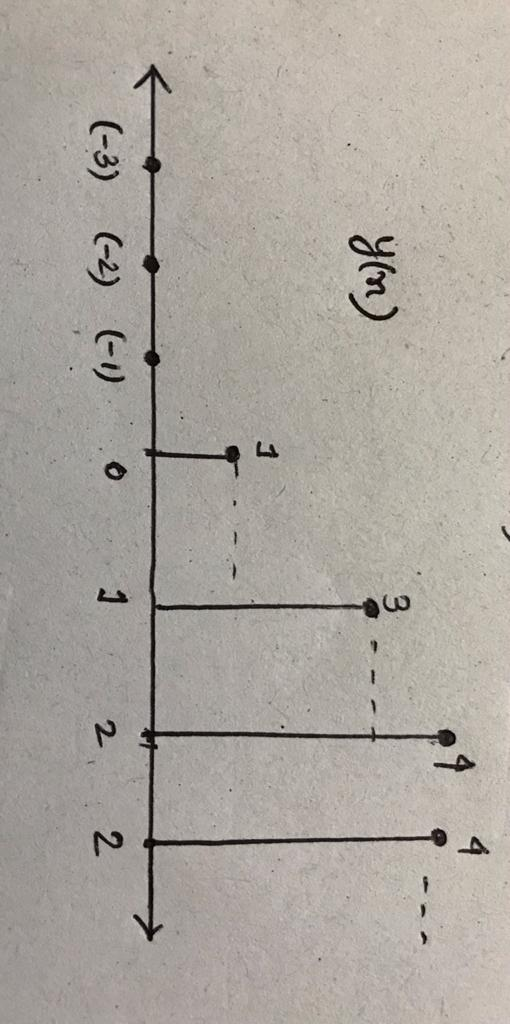
\includegraphics[height = 0.5\linewidth, angle = 90]{q7_a.jpeg}
        \end{figure}

        \item[(b)] We are given;
        $$
        x(n) = [1, 2, \underset{\uparrow}{1}, 1, 2] \qquad h(n) = \delta(n+2)
        $$

        In this case, as $h(n) \neq 0$ only if $n = (-2)$,

        $$
        y(n) = \sum_{k = -\infty}^{\infty} h(k)x(n-k) = x(n+2)
        $$

        Thus, $y(n) = [1, 2, 1, 1, \underset{\uparrow}{2}]$.

        \begin{figure}[H]
            \centering
            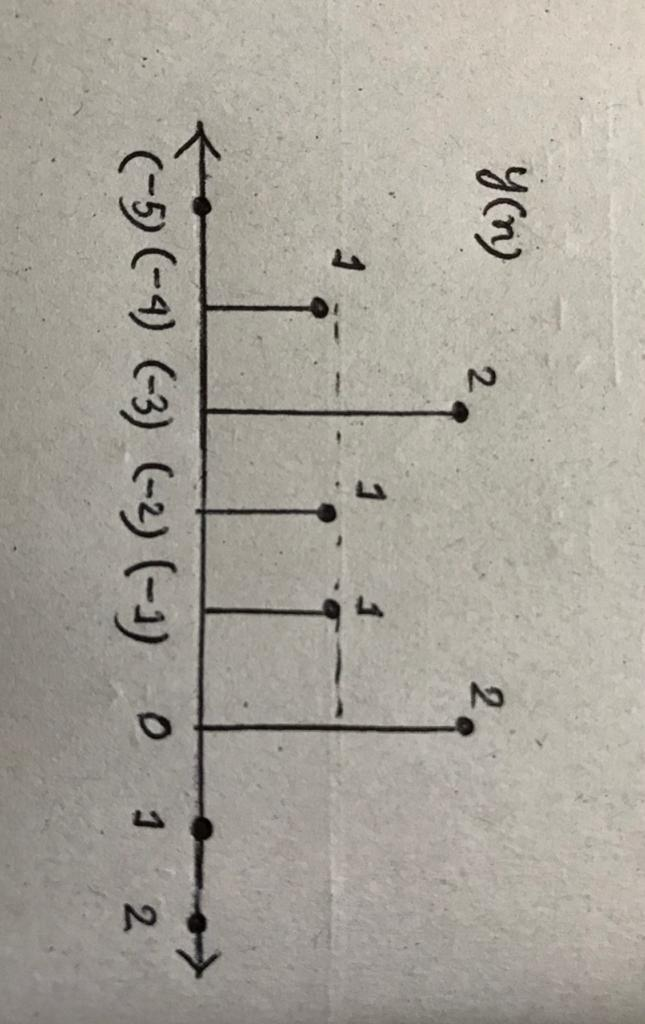
\includegraphics[height = 0.5\linewidth, angle = 90]{q7_b.jpeg}
        \end{figure}
        
        \item[(c)] We are given; 
        $$
        x(n) = \alpha^n u(n) \qquad h(n) = \beta^n u(n); \qquad 0 < \alpha \neq \beta < 1
        $$ 

        Now,

        \begin{align*}
            y(n) 
            & = (h \ast x)(n) \\
            & = \sum_{k = -\infty}^{\infty} x(k)h(n-k)\\
            & = \sum_{k = -\infty}^{\infty} \alpha^k \beta^{(n-k)} u(k)u(n-k)\\
            & = \beta^n + \alpha \beta^{(n-1)} + \alpha^2 \beta^{(n-2)} + \dots + \alpha^{(n-1)}\beta + \alpha^n \qquad \text{ assume, } n \geq 0\\
            & = \dfrac{(\beta^{(n+1)} - \alpha^{(n+1)})}{(\beta - \alpha)}
        \end{align*}

        On the other hand, if $n < 0$, clearly $y(n) = 0$. Thus,
        $$
        y(n) = \dfrac{(\beta^{(n+1)} - \alpha^{(n+1)})}{(\beta - \alpha)} u(n)
        $$

        The sketch of the signal looks as follows:

        \begin{figure}[H]
            \centering
            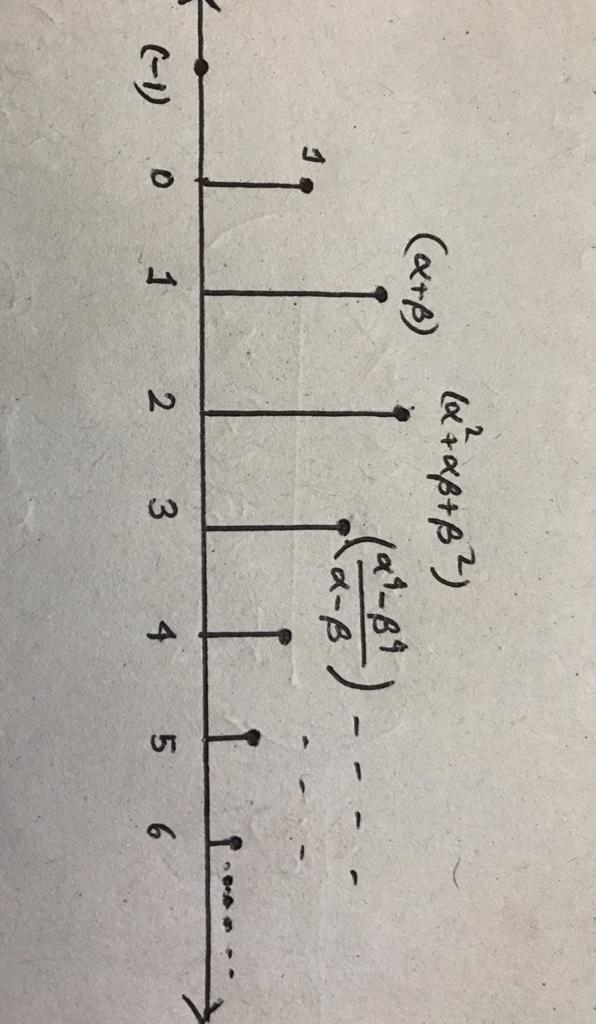
\includegraphics[height = 0.5\linewidth, angle = 90]{q7_c.jpeg}
        \end{figure}        
    \end{enumerate}
\end{answer}




% DONE
\begin{question}
    In this problem we wish to show that for an LTI system a necessary and sufficient condition for causality is that the unit sample response be zero for $n < 0$.
    \begin{enumerate}
        \item[(a)] Show from the convolution sum that if $h(n) = 0$ for $n < 0$, then the system must be causal, i.e. that $y(n_0)$ depends only on $x(n)$ for $n \leq n_0$ where $n_0$ is arbitrary. This then shows that a sufficient condition for causality of an LTI system is that $h(n) = 0$, $n < 0$.
        \item[(b)] Now, suppose that $h(n)$ is not zero for $n < 0$. Argue that the system cannot be causal. This can be done simply by showing that there is at least one input for which the output "anticipates" the input i.e. for which $y(n_0)$ depends on values of $x(n)$ for $n > n_0$. This then establishes that a necessary condition for causality of an LSI system is that $h(n) = 0$, $n < 0$. 
    \end{enumerate} 
\end{question}

\begin{answer}
    We wish to show that a necessary and sufficient condition for an LTI system to be causal is that its unit sample response is zero for $n < 0$.
    \begin{enumerate}
        \item[(a)] First, we assume that the unit sample response $h(n)$ satisfies, $h(n) = 0$ for any $n < 0$. Now for any arbitrary integer $n_0$ and by the discrete convolution characterization of an LTI system,
        \begin{align*}
            y(n_0) 
            & = (h \ast x)(n_0) \qquad \text{ where } \ast \text{ denotes discrete convolution}\\
            & = \sum_{n = -\infty}^{\infty} h(n)x(n_0 - n)\\
            & = \sum_{n = -\infty}^{-1} h(n)x(n_0 - n) + \sum_{n = 0}^{\infty} h(n)x(n_0 - n)\\
            & = \sum_{n = 0}^{\infty} h(n)x(n_0 - n) \qquad \text{since, } h(n) = 0 \quad \forall n < 0\\
            & = h(0)x(n_0) + h(1)x(n_0 - 1) + h(2)x(n_0 - 2) + \dots
        \end{align*}

        This shows that current output $y(n_0)$ is simply a linear combination of the current and past input values, where the coefficients are given by the values of unit sample response sequence $h(n)$. Thus, the system is \textbf{causal}.

        \item[(b)] Now conversely, suppose $h(n_0) \neq 0$ for some $n_0 < 0$. Consider any arbitrary sequence $x(n)$ and assume that we input $z(n) = x(n)\delta(n + n_0)$ into the system. Then,
        
        \begin{align*}
            y(0) 
            & = \sum_{k = -\infty}^{\infty} h(k)z(-k)\\
            & = h(n_0) x(-n_0)  \qquad \text{since, } z(n) = 0 \quad \forall n \neq (-n_0)\\
        \end{align*}

        Since, $n_0 < 0$, thus $(-n_0) > 0$ and hence $y(0)$ depends on a future input $x(-n_0)$. This shows that the system is \textbf{noncausal}.
    \end{enumerate}
\end{answer}


% DONE
\begin{question}
    The discrete-time system $y(n) = ny(n - 1) + x(n)$, $n \geq 0$, is at rest [i.e. $y(-1) = 0$]. Check if the system is linear time invariant and BIBO stable.     
\end{question}

\begin{answer}
    We have the discrete time system $y(n) = n y(n-1) + x(n)$ for any $n \geq 0$. Putting $n = 0$ yields, $y(0) = x(0)$.

    Note that,
    \begin{align*}
        y(n) - n y(n-1) & = x(n)\\
        ny(n-1) - n(n-1) y(n-2) & = nx(n-1)\\
        n(n-1) y(n-2) - n(n-1)(n-2) y(n-3) & = n(n-1)x(n-2)\\
        \dots & \dots\\
        n! y(1) - n! y(0) & = n! x(1)\\
        n!y(0) & = n! x(0)
    \end{align*}

    where $n!$ is the quantity obtained by multiplying all natural numbers upto $n$. Adding all these quantities yield; 

    $$
    y(n) = x(n) + nx(n-1) + n(n-1)x(n-2) + \dots + n! x(0) = \sum_{k = 0}^{n} \dfrac{n!}{k!} x(k)
    $$

    Notice that, the system is \textbf{linear}, as for any arbitrary sequences $x_1(n)$ and $x_2(n)$, and for any $\alpha, \beta \in \R$ (assume $\tau$ denotes the system);

    \begin{align*}
        \tau(\alpha x_1(n) + \beta x_2(n)) 
        & = \sum_{k = 0}^{n} \dfrac{n!}{k!} (\alpha x_1(k) + \beta x_2(k)) \\
        & = \alpha \sum_{k = 0}^{n} \dfrac{n!}{k!} x_1(k) + \beta \sum_{k = 0}^{n} \dfrac{n!}{k!} x_2(k)\\
        & = \alpha \tau(x_1(n)) + \beta \tau(x_2(n))
    \end{align*}

    The given system is \textbf{time varying}, for instance, consider the input $x(n) = [\underset{\uparrow}{1}, 2, 3]$ to the system, which outputs $y(n) = [\underset{\uparrow}{1}, 3, 9]$. Now, consider inputting the delayed version of $x(n)$ i.e. $[1, \underset{\uparrow}{2}, 3]$ to the system, which outputs $[0, \underset{\uparrow}{2}, 5]$, which is not a delayed version of $y(n)$.

    Finally, the system is \textbf{BIBO unstable}. For this, consider the bounded input sequence $x(n) = u(n)$. Then, 
    
    $$
    y(n) = n! \sum_{k = 0}^{n} \dfrac{u(k)}{k!} \geq n! \times \dfrac{1}{0!} = n!
    $$

    where the sequence $n!$ is unbounded. Hence, $y(n)$ is also unbounded.
\end{answer}




\begin{question}
    Consider the system $y(n) = \tau[x(n)] = x(n^2)$.
    \begin{enumerate}
        \item[(a)] Determine if the system is time invariant.
        \item[(b)] To clarify the result in part (a), assume that the signal;
        $$
        x(n) = \begin{cases}
            1 & 0 \leq n \leq 3\\
            0, & \text{ elsewhere}
        \end{cases}
        $$  
        is applied to the system.
        \begin{enumerate}
            \item[(1)] Sketch the signal $x(n)$.
            \item[(2)] Determine and sketch the signal $y(n) = \tau[x(n)]$.
            \item[(3)] Sketch the signal $y'_2(n) = y(n-2)$.
            \item[(4)] Determine and sketch the signal $x_2(n) = x(n-2)$.
            \item[(5)] Determine and sketch the signal $y_2(n) = \tau[x_2(n)]$.
            \item[(6)] Compare the signals $y_2(n)$ and $y(n-2)$. What is your conclusion?
        \end{enumerate}
        \item[(c)] Repeat part (b) for the system $y(n) = x(n) - x(n-1)$. Can you use this result to make any statement about the time invariance of the system? Why?
        \item[(d)] Repeat parts (b) and (c) for the system $y(n) = \tau[x(n)] = nx(n)$. 
    \end{enumerate}
\end{question}


\begin{answer}
    \begin{enumerate}
        \item[(a)] The system is \textbf{not time invariant}. Consider any integer $n_0$, then with $y(n) = \tau(x(n)) = x(n^2)$, and with a delayed version of $x(n)$ as the input signal, we have;
        
        $$
        \tau(x(n - n_0)) = x((n - n_0)^2) \neq x(n^2 - n_0) = y(n - n_0)
        $$
    
        Thus, in general as $((n - n_0)^2)$ and $(n^2 - n_0)$ are different for arbitrary $n$ and $n_0$, the above inequality would be true and the system will remain \textbf{time varying}.
    
        \item[(b)] We have,
        \begin{align*}
            x(n) & = [\underset{\uparrow}{1}, 1, 1, 1]\\
            y(n) = \tau[x(n)] & = [1, \underset{\uparrow}{1}, 1]\\
            y'_2(n) = y(n-2) & = [\underset{\uparrow}{0}, 1, 1, 1]\\
            x_2(n) = x(n-2) & = [\underset{\uparrow}{0}, 0, 1, 1, 1]\\
            y_2(n) = \tau[x_2(n)] & = [1, 0, \underset{\uparrow}{0}, 0, 1]\\
        \end{align*} 
        The sketches are shown below.
        \begin{figure}[H]
            \centering
            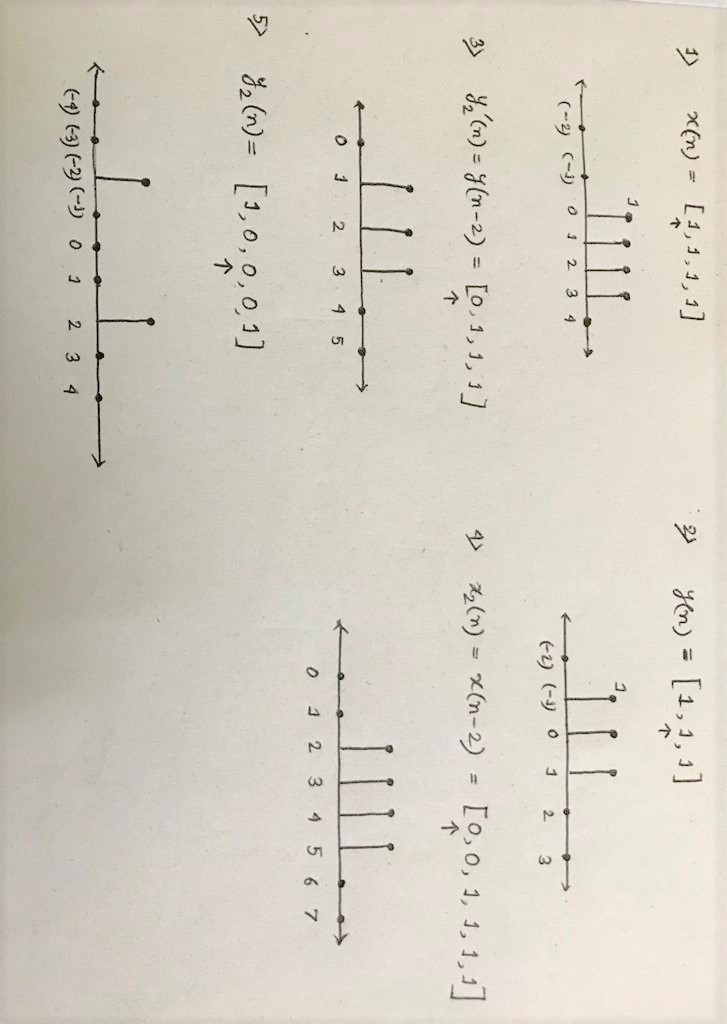
\includegraphics[height= \linewidth, angle = 90]{q10_b.jpeg}
        \end{figure} 

        Clearly, $y'_2(n) \neq y_2(n)$, thus there is at least one input $x(n)$ as given above such that a delayed version of $x(n)$ if passed as input to the system does not output a delayed version of the corresponding output $y(n)$, hence the system is \textbf{time varying}.

        \item[(c)] We have,
        \begin{align*}
            x(n) & = [\underset{\uparrow}{1}, 1, 1, 1]\\
            y(n) = \tau[x(n)] & = [\underset{\uparrow}{1}, 0, 0, 0, (-1)]\\
            y'_2(n) = y(n-2) & = [\underset{\uparrow}{0}, 0, 1, 0, 0, 0, (-1)]\\
            x_2(n) = x(n-2) & = [\underset{\uparrow}{0}, 0, 1, 1, 1]\\
            y_2(n) = \tau[x_2(n)] & = [\underset{\uparrow}{0}, 0, 1, 0, 0, 0, (-1)]\\
        \end{align*} 
        The sketches are shown below.
        \begin{figure}[H]
            \centering
            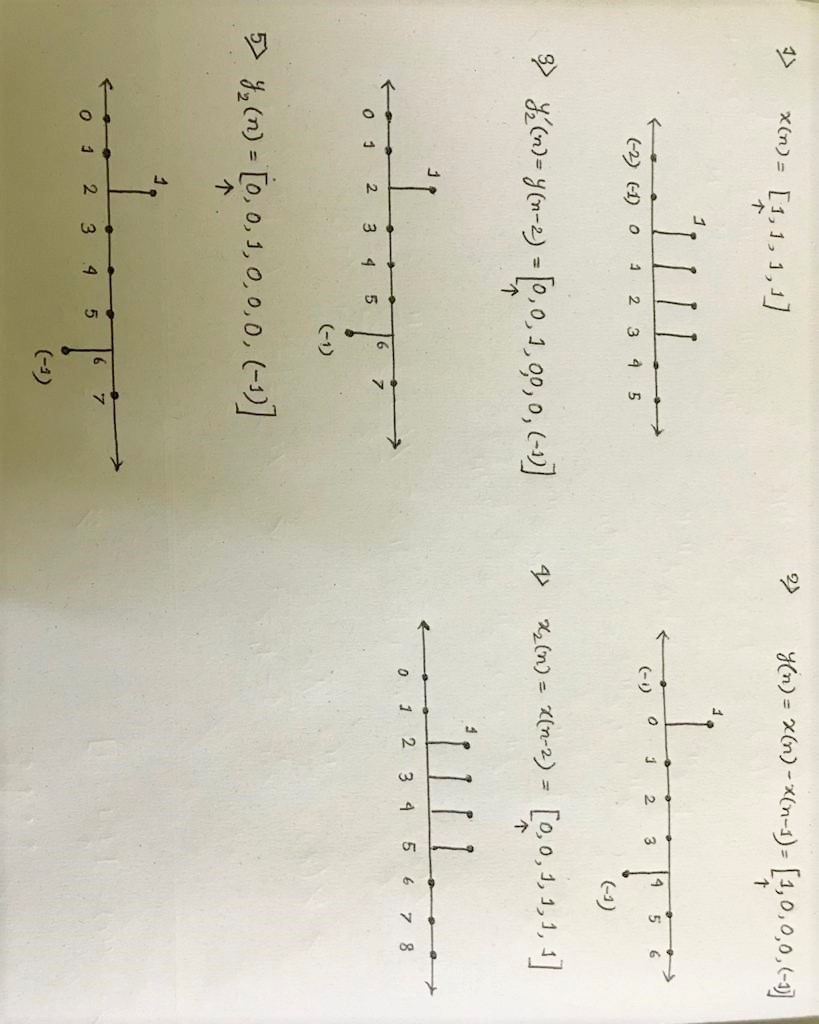
\includegraphics[height= \linewidth, angle = 90]{q10_c.jpeg}
        \end{figure}

        This shows that for this particular input $x(n)$, if a delayed version of the input is fed to the system, a delayed version of the corresponding output $y(n)$ is obtained. However, this is not enough to draw any kind of conclusion about the system. Since, there might be some other sequence where this property is failed, and then the system will be time varying, however, if no other input sequence violates this property, the system will be time invariant.

        \item[(d)] For the given system $y(n) = nx(n)$, we have;
        \begin{align*}
            x(n) & = [\underset{\uparrow}{1}, 1, 1, 1]\\
            y(n) = \tau[x(n)] & = [\underset{\uparrow}{0}, 1, 2, 3]\\
            y'_2(n) = y(n-2) & = [\underset{\uparrow}{0}, 0, 0, 1, 2, 3]\\
            x_2(n) = x(n-2) & = [\underset{\uparrow}{0}, 0, 1, 1, 1]\\
            y_2(n) = \tau[x_2(n)] & = [\underset{\uparrow}{0}, 0, 2, 3, 4, 5]\\
        \end{align*} 
        The sketches are shown below.
        \begin{figure}[H]
            \centering
            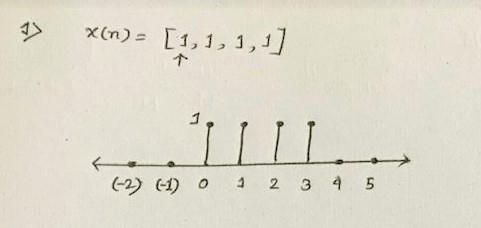
\includegraphics[width= 0.55\linewidth]{q10_d_1.jpeg}
            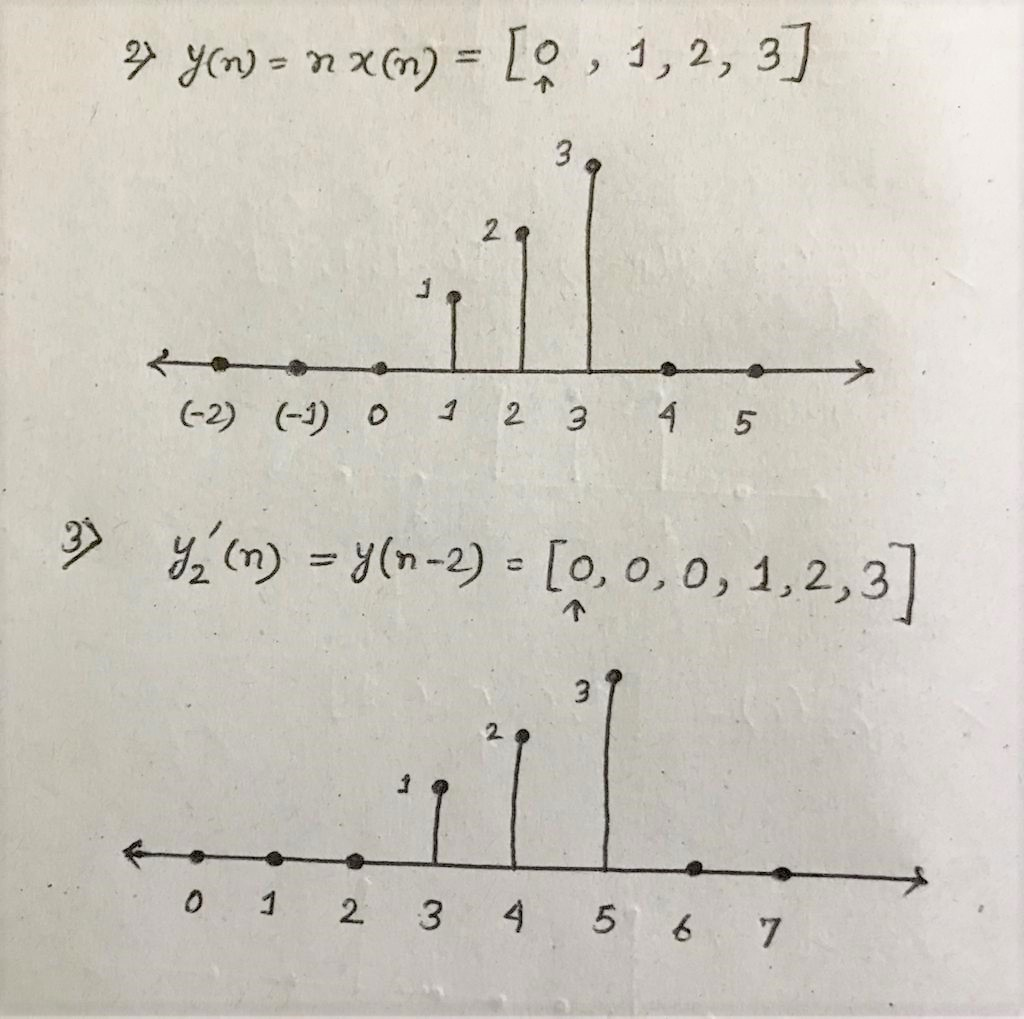
\includegraphics[width= 0.55\linewidth]{q10_d_2.jpeg}
        \end{figure}

        \begin{figure}[H]
            \centering
            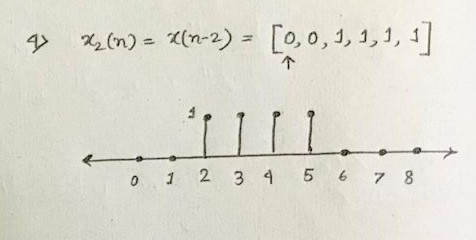
\includegraphics[width = 0.6\linewidth]{q10_d_4.jpeg}
            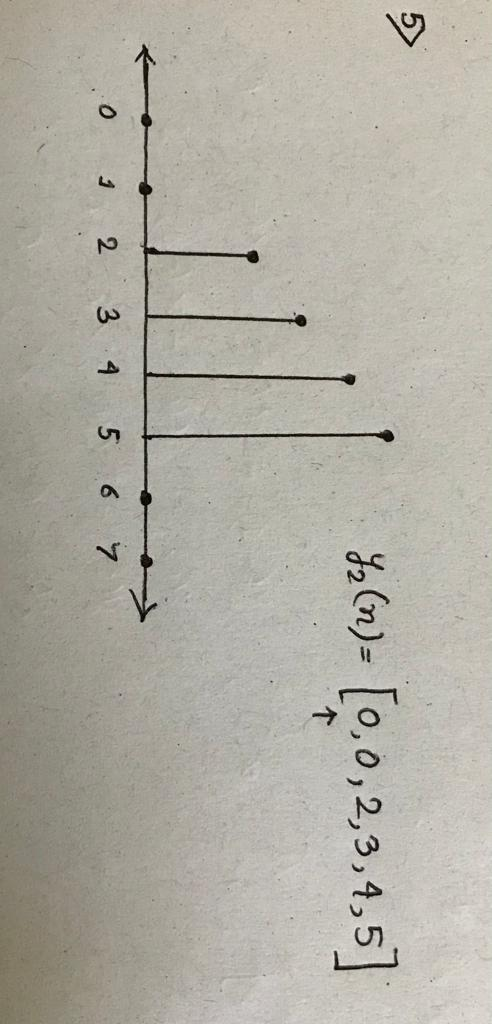
\includegraphics[height = 0.6\linewidth, angle = 90]{q10_d_5.jpeg}
        \end{figure}

        Clearly again, $y'_2(n) \neq y_2(n)$, thus there is at least one input $x(n)$ as given above such that a delayed version of $x(n)$ if passed as input to the system does not output a delayed version of the corresponding output $y(n)$, hence the system is \textbf{time varying}.
    \end{enumerate}    
\end{answer}


\end{document}
